\section{Cluster Analysis} \label{sect:analysis}

Now that we have built up an understanding of how CNRE behaves, we move to
investigate the aggregate catchments of clients using clustering techniques
discussed in the previous section. In this section, we use the discussed
CNRE threshold of 0.73 for cluster formation. This threshold yields 870 clusters
with a median cluster size of REF.

\begin{figure}
    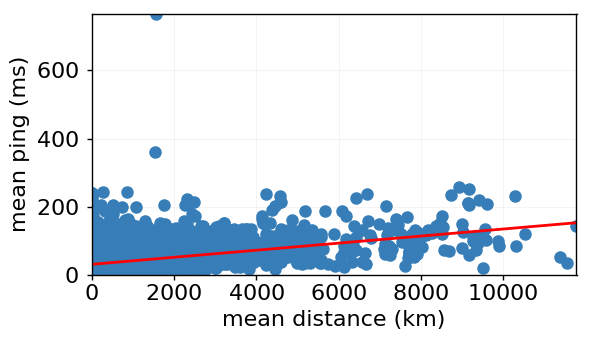
\epsfig{file=figs/geo_vs_perf.png, width=1\linewidth}
    \caption{CDF of \# of outliers per cluster for geo distance, etc}
\end{figure}

In 

\begin{figure}
    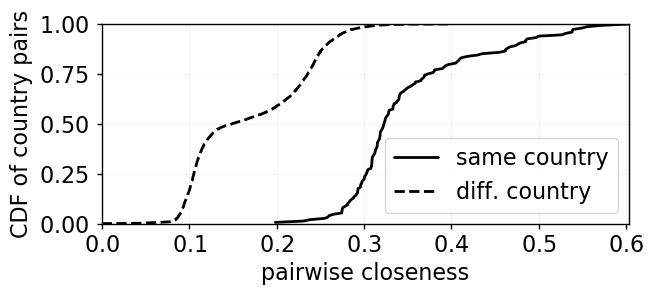
\epsfig{file=figs/country_cdf.png, width=1\linewidth}
    \caption{Domain match alignment with clusters (what format?)}
\end{figure}

\begin{figure}
    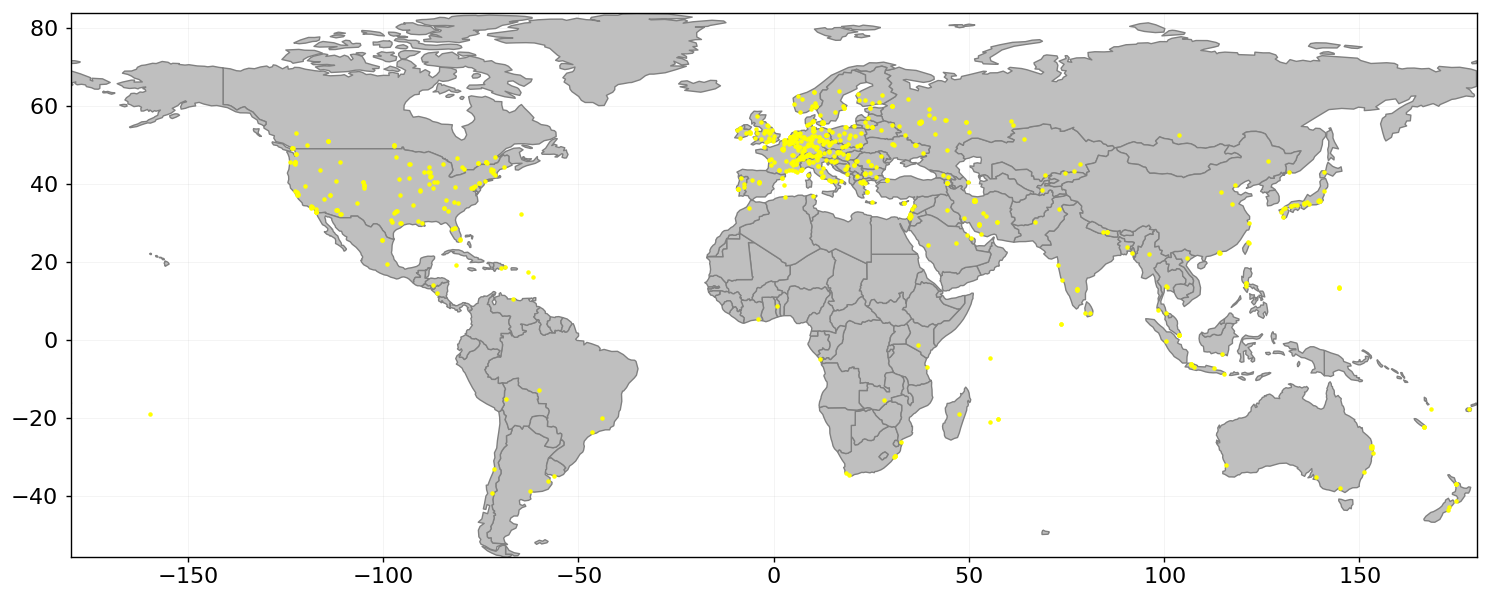
\epsfig{file=figs/geo_centers.png, width=1\linewidth}
    \caption{Map of world with point for each cluster's geographic center.}
\end{figure}

